%============================ MAIN DOCUMENT ================================
\PassOptionsToPackage{table}{xcolor}
\documentclass[
  a4paper,
  invert-title,
  titleimage-ratio=13
]{bfhpub}

\usepackage[french,english,main=ngerman]{babel}  % https://www.namsu.de/Extra/pakete/Babel.html
\LoadBFHModule{listings,terminal,boxes}
%---------------------------------------------------------------------------
% Documents paths
%---------------------------------------------------------------------------
\makeatletter
\def\input@path{{content/}}
%or: \def\input@path{{/path/to/folder/}{/path/to/other/folder/}}
\makeatother
%-----------------  Base packages     --------------------------------------
% Include Packages
\usepackage{amsmath}          % various features to facilitate writing math formulas
\usepackage{amsthm}           % enhanced version of latex's newtheorem
\usepackage{amsfonts}         % set of miscellaneous TeX fonts that augment the standard CM
\usepackage{amssymb}          % mathematical special characters

\usepackage{siunitx}

\usepackage{graphicx}         % integration of images
\usepackage{float}            % floating objects

\usepackage{caption}          % for captions of figures and tables
\usepackage{subcaption}       % for subcaptions in subfigures
\usepackage{cite}             % use bibtex
\usepackage{wrapfig}

\usepackage{exscale}          % mathematical size corresponds to textsize
\usepackage{multirow}         % multirow emables combining rows in tables
\usepackage{multicol}

\usepackage{longtable}
\usepackage{adjustbox}

%---------------------------------------------------------------------------
% Graphics paths
%---------------------------------------------------------------------------
\graphicspath{{pictures/}{figures/}}
%---------------------------------------------------------------------------
% Blind text -> for dummy text
%---------------------------------------------------------------------------
\usepackage{blindtext}    
\usepackage{letltxmacro}   
\LetLtxMacro{\blindtextblindtext}{\blindtext}

\RenewDocumentCommand{\blindtext}{O{\value{blindtext}}}{
	\begingroup\color{BFH-Gray}\blindtextblindtext[#1]\endgroup
}
%---------------------------------------------------------------------------
% Glossary Package
%---------------------------------------------------------------------------
% the glossaries package uses makeindex
% if you use TeXnicCenter do the following steps:
%  - Goto "Ausgabeprofile definieren" (ctrl + F7)
%  - Select the profile "LaTeX => PDF"
%  - Add in register "Nachbearbeitung" a new "Postprozessoren" point named Glossar
%  - Select makeindex.exe in the field "Anwendung" ( ..\MiKTeX x.x\miktex\bin\makeindex.exe )
%  - Add this [ -s "%tm.ist" -t "%tmx.glg" -o "%tm.gls" "%tm.glo" ] in the field "Argumente"
%
% for futher informations go to http://ewus.de/tipp-1029.html
%---------------------------------------------------------------------------
\usepackage[nonumberlist]{glossaries-extra}
\makeglossaries
%----------------  Glossary Entries  ---------------------------------------
\newglossaryentry{latex}{
    name=LaTeX,
    description={Ein Textsatzsystem für wissenschaftliche Dokumente}
}

\newglossaryentry{bfh}{
    name=BFH,
    description={Berner Fachhochschule}
}

%----------------  Acronyms  -----------------------------------------------
\newacronym{ai}{AI}{Artificial Intelligence}
\newacronym{ml}{ML}{Machine Learning}
%---------------------------------------------------------------------------
% Makeindex Package
%---------------------------------------------------------------------------
\usepackage{makeidx}
\makeindex
%\usepackage{imakeidx}          % To produce index
%\makeindex[columns=2,intoc]    % Index-Initialisation
%\makeindex[columns=3,columnseprule,columnsep,intoc]
%---------------------------------------------------------------------------
% Hyperref Package (Create links in a pdf)
%---------------------------------------------------------------------------
\usepackage[
	,bookmarks
	,plainpages=false
	,pdfpagelabels
    ,pdfusetitle
	,backref = {false}          % No index backreference
	,colorlinks = {true}        % Color links in a PDF
	,hypertexnames = {true}     % no failures "same page(i)"
	,bookmarksopen = {true}     % opens the bar on the left side
	,bookmarksopenlevel = {0}   % depth of opened bookmarks
	,linkcolor=.
	,filecolor=.
	,urlcolor=.
	,citecolor=.
]{hyperref}
%---------------------------------------------------------------------------

%% %% Customize Footer and Headers in Document
%% \KOMAoptions{headsepline,plainheadsepline,footsepline,plainfootsepline}%
%% \setkomafont{headsepline}{\color{BFH-DarkBlue}}% BFH-DarkBlue required bfhcolors
%% \setkomafont{footsepline}{\color{BFH-DarkBlue}}%
%% \lehead*{lehead} % the * character does replace the header on the first chapter page as well
%% \cehead*{cehead}
%% \rehead*{rehead}
%% \lohead*{lohead}
%% \cohead*{cohead}
%% \rohead*{rohead}

%% \lefoot*{lefoot}
%% \cefoot*{cefoot}
%% \refoot*{refoot}
%% \lofoot*{lofoot}
%% \cofoot*{cofoot}
%% \rofoot*{rofoot}
%---------------------------------------------------------------------------
\begin{document}

%% Snippet do redefine German babel translations -- see FAQ latex.ti.bfh.ch for further information or
%% the package documentation https://www.ctan.org/pkg/translations
%% \redefinetranslation{German}{Advisor}{Dozentin}
%% \redefinetranslation{German}{advisor}{Dozentin} %  just for consistency
%% \redefinetranslation{German}{Author}{Autorin}
%% \redefinetranslation{German}{author}{Autorin} %  just for consistency
%% \redefinetranslation{German}{Co-advisor}{Mitbetreuerin}
%% \redefinetranslation{German}{co-advisor}{Mitbetreuerin} %  just for consistency
%% \redefinetranslation{German}{Expert}{Expertin}
%% \redefinetranslation{German}{expert}{Expertin} %  just for consistency
%% \redefinetranslation{German}{Project partner}{Projektpartnerin}
%% \redefinetranslation{German}{project partner}{Projektpartnerin} %  just for consistency
%------------ Translations -------------------------------------------------------------------------------------------------------------------------------
%------------ Additional commands ------------------------------------------------------------------------------------------------------------------------

%------------ START FRONT PART ---------------------------------------------------------------------------------------------------------------------------
\frontmatter % Nummerierung der Seiten in römischen Zahlen

%----------------  BFH tile page   -----------------------------------------
  \title{Projekt 4: Kombinatorische Logik}
  \subtitle{BTE5213 Laborprojekte, Herbstsemester 2025/2026\\Protokoll}
  \author{Janis Aebischer \and Simon Eisele}
  \department{Technik und Informatik}
  \institute{Elektrotechnik und Informationstechnologie}
  \version{1.0}
  \titlegraphic{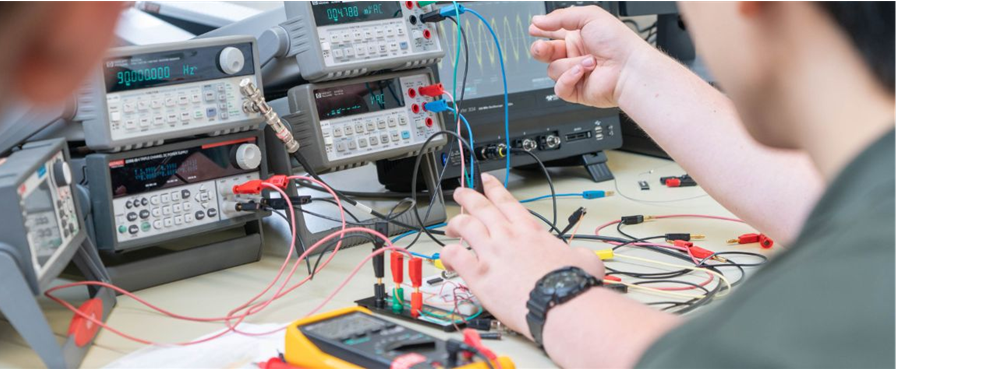
\includegraphics{Bild1.png}}
  \maketitle

%------------ ABSTRACT        ----------------
\section{Abstract}
One-paragraph summary of the entire study – typically no more than 250 words in length (and in many cases it is well shorter than that), the Abstract provides an overview of the study.

%------------ TABLEOFCONTENTS ----------------
\tableofcontents

%------------ START MAIN PART ------------
\mainmatter

%------------ Introduction ------------
\clearpage
\section{Einleitung}
\section{Introduction}

What is the topic and why is it worth studying? – the first major section of text in the paper, the Introduction commonly describes the topic under investigation, summarizes or discusses relevant prior research (for related details, please see the Writing Literature Reviews section of this website), identifies unresolved issues that the current research will address, and provides an overview of the research that is to be described in greater detail in the sections to follow.

\clearpage
\section{Methoden und Materialien}

\clearpage
\section{Resultate}
\section{Results}
What did you find? – a section which describes the data that was collected and the results of any statistical tests that were performed.  It may also be prefaced by a description of the analysis procedure that was used. If there were multiple experiments, then each experiment may require a separate Results section.

\clearpage
\section{Diskussion}
Ziel des Abschnitts Diskussion ist es die Ergebnisse des Versuchs zusammenzufassen und zu reflektieren.
–	Erreichte Funktionalität und verbleibende Probleme
–	Fazit und Reflexion
%------------ Authorship declaration translated to main language ------------
%\declarationOfAuthorship

%----------- Bibliography ----------------
\clearpage
\bibliographystyle{unsrt}
\bibliography{project}      % the project.bib file gets loaded

%------------ List of Figures ------------
\listoffigures
 
%------------ List of Tables -------------
\listoftables
 
%------------ List of Listings -----------
\lstlistoflistings 
 
%------------ Glossary -------------------
\printglossary

%------------ Index ----------------------
\clearpage
\printindex
%------------ Appendix ----------------	
\appendix
%\chapter{First Appendix Chapter}

\end{document}
